\documentclass[12pt]{article}
\usepackage[spanish]{babel}
\usepackage[utf8]{inputenc}
\usepackage[T1]{fontenc}
\usepackage{geometry}
\usepackage{fancyhdr}
\usepackage{graphicx}
\usepackage{float}
% Configuración de márgenes
\geometry{a4paper, left=2.5cm, right=2.5cm, top=3cm, bottom=3cm}

% Configuración de encabezado y pie de página
\pagestyle{fancy}
\fancyhf{}
\lhead{Proyecto 1 Sistemas Operativos}
\cfoot{\thepage}

\begin{document}

\title{Proyecto 1}
\author{Roberto Artigues, Emilio Meza, Nicolás Soto}
\date{8 de Octubre de 2023}
\maketitle


\section{Introducción}
Desarrollo de un intérprete de comandos simple en Linux (shell). La shell a implementar será similar
a las disponibles actualmente en Linux.
\section{Parte 1}
En el main del codigo se pueden visualizar todos los procesos solicitados para este proyecto, 
cada uno comentado para que sea mas fácil su entendimiento.


\section{Parte 2}
Se creo la funcion a continuacion, con sus comentarios en el código explicando los pasos que sigue.
\begin{figure}[H]
    \centering
    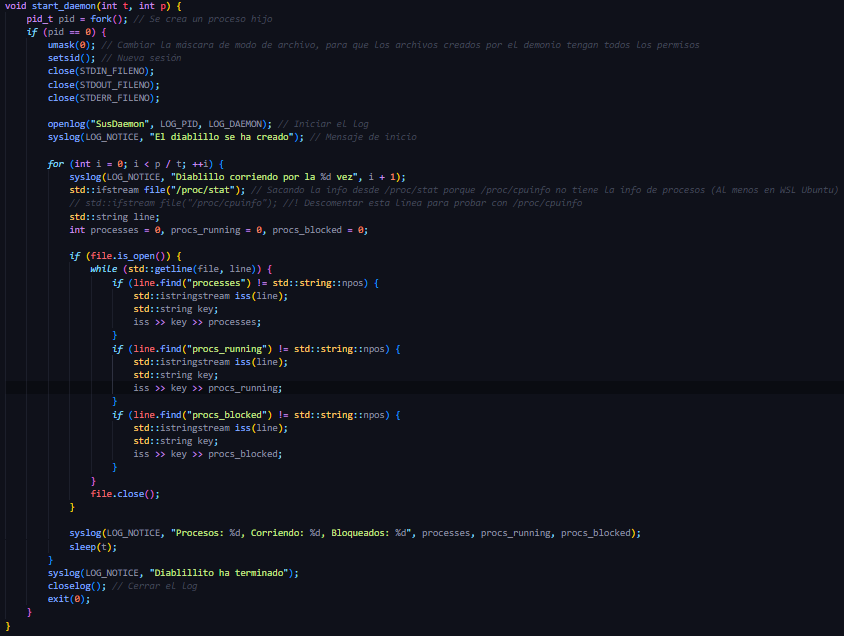
\includegraphics[width=0.7\textwidth]{daemon.png}
    \caption{Funcion Demonio}
\end{figure}
\begin{figure}[H]
    \centering
    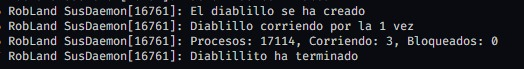
\includegraphics[width=0.7\textwidth]{demonio-working.jpeg}
    \caption{Demonio haciendo sus procesos}
\end{figure}

\end{document}